%presentation.tex
%Andy Sayler
%Constantin Berzan
%-----------------------------------------------------------------------------%
\documentclass[xcolor=dvipsnames]{beamer}
%\useoutertheme{default}
%\usetheme{Boadilla}
\setbeamercovered{transparent=25}
\setbeamertemplate{blocks}[rounded][shadow=false] 
\setbeamertemplate{navigation symbols}{}
\usepackage{graphics}
\usepackage{url}

\title[SLAM]{Videre SLAM}
%\subtitle[]{}
\author[ C. Berzan \& A. Sayler]{ Constantin Berzan \& Andy Sayler}
\institute[Tufts University]{
  Tufts University\\
  COMP150 - BBR\\
  \texttt{constantin.berzan@tufts.edu}\\*
  \texttt{andrew.sayler@tufts.edu}
}
\date[Dec. 14, 2010]{Tuesday, December 14\textsuperscript{th}, 2010}

\begin{document}
  
  %----Title Slide------------------------------------------------------------%
  \begin{frame}[plain]
    \titlepage
  \end{frame}
  
  \section*{Outline}  
  %----Outline Slide----------------------------------------------------------%
  \begin{frame}{\bf Outline}
    %\pause
    \tableofcontents[]
  \end{frame}
  
  \section{Overview}
  %----SLAM Overview - Andy--------------------------------------------------%
  \begin{frame}{\bf SLAM Overview}
    \begin{columns}[t]
      \begin{column}{0.5\textwidth}

        {\bf S}imultaneous \\*
        {\bf L}ocation \\*
        {\bf A}nd \\*
        {\bf M}apping \\*

        \vspace{1cm}

        SLAM is a methodology for implementing location awareness on a mobile platform.
      \end{column}
      \begin{column}{0.5\textwidth}
        \begin{figure}
          \begin{center}
            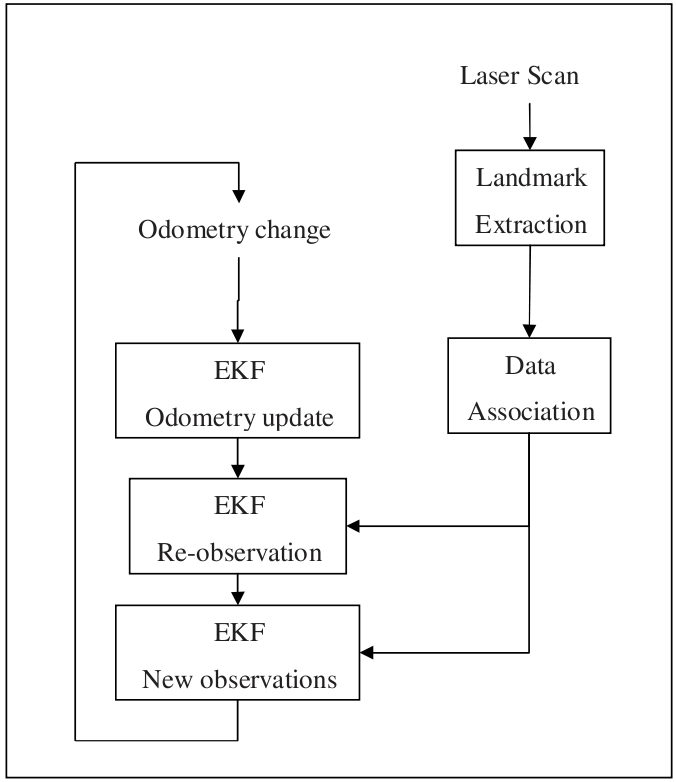
\includegraphics[scale=.3]{slamoverview.png}
          \end{center}
          \caption{Slam Overview \cite{SlamForDummies}}
          \label{fig:slamoverview}
        \end{figure}
      \end{column}
    \end{columns}
  \end{frame}
  
  \section{Landmarks}
  %----Landmarks - Constantin--------------------------------------------------%
  \begin{frame}{\bf Landmark Extraction}

    Landmarks: easily reobservable features in the environment, used in
    localization
    \vspace{1cm}

    Our landmark extraction algorithm:
    \begin{itemize}
    \item Extract lines from laser readings (RANSAC)
    \item Determine the origin of the world coordinate system using the
          estimated robot position
    \item Project origin onto each line, take resulting points as landmarks
    \end{itemize}
    \vspace{1cm}

    Landmarks are passed to the EKF only after they have been seen several
    times. Old landmarks that have not been seen in a while are ``forgotten.''
  \end{frame}

  \begin{frame}{\bf Line Extraction}

    RANSAC: Random Sample Consensus
    \vspace{0.5cm}

    Input: set of points $\mathcal{P}$

    Output: set of fitted lines $\mathcal{L}$

    Algorithm:
    \begin{itemize}
    \item Select random subset of points $\mathcal{P}_{sample}$
    \item Fit line $\ell_{sample}$ through sample points
    \item Compute set $\mathcal{P}_{consensus}$ of all points in $\mathcal{P}$
          that are within a small distance of the line $\ell_{sample}$
    \item If there are enough such points, fit a new line
          $\ell_{consensus}$ through $\mathcal{P}_{consensus}$.
          Add $\ell_{consensus}$ to the output set $\mathcal{L}$, and
          remove all fitted points $\mathcal{P}_{consensus}$ from $\mathcal{P}$
    \item Repeat until all points are fitted, or a maximum number of iterations
          is reached
    \end{itemize}
  \end{frame}

  {
  \usebackgroundtemplate{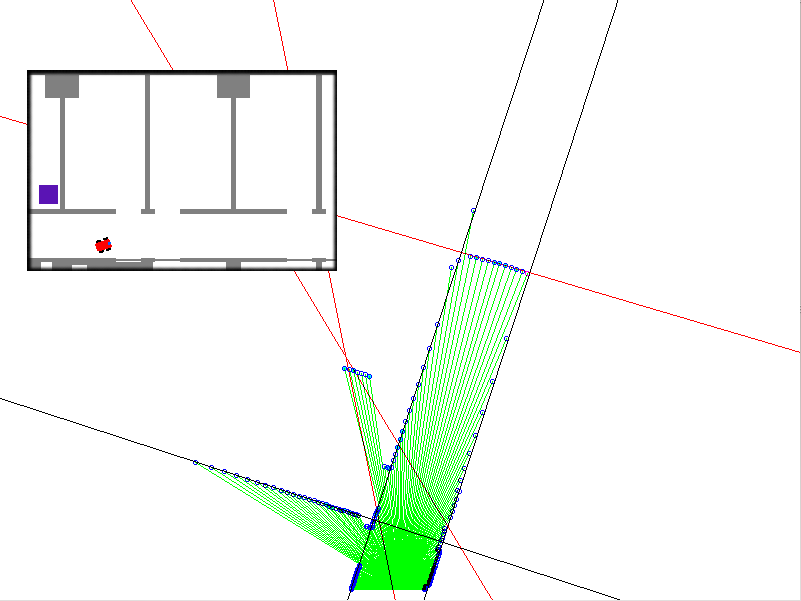
\includegraphics[width=\paperwidth]{ransac-mix.png}}
  \begin{frame}{}
  \end{frame}
  }

  {
  \usebackgroundtemplate{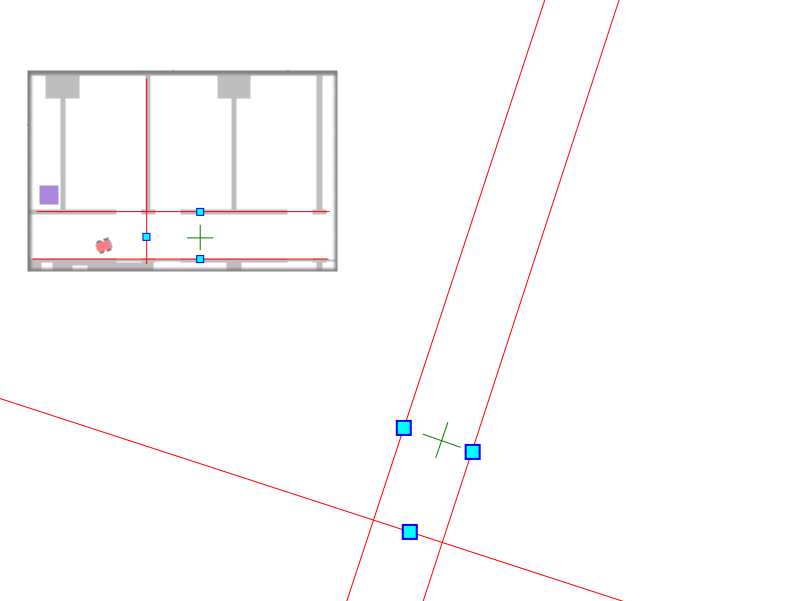
\includegraphics[width=\paperwidth]{landmark-mix.png}}
  \begin{frame}{}
  \end{frame}
  }

  \section{EKF}
  %----EKF - Andy--------------------------------------------------%
  \begin{frame}{\bf EKF}

    Extended Kalman Filter: Linearized method for distilling ``true''
    values from noisy measurements.
    
    Two main steps:
    \begin{itemize}
    \item {\bf Prediction}: Use system model to predict value of next
    measurement
    \item {\bf Update}: Take noisy measurement and use it to refine the
      estimation of the true value
    \end{itemize}
    
  \end{frame}

  {
    \usebackgroundtemplate{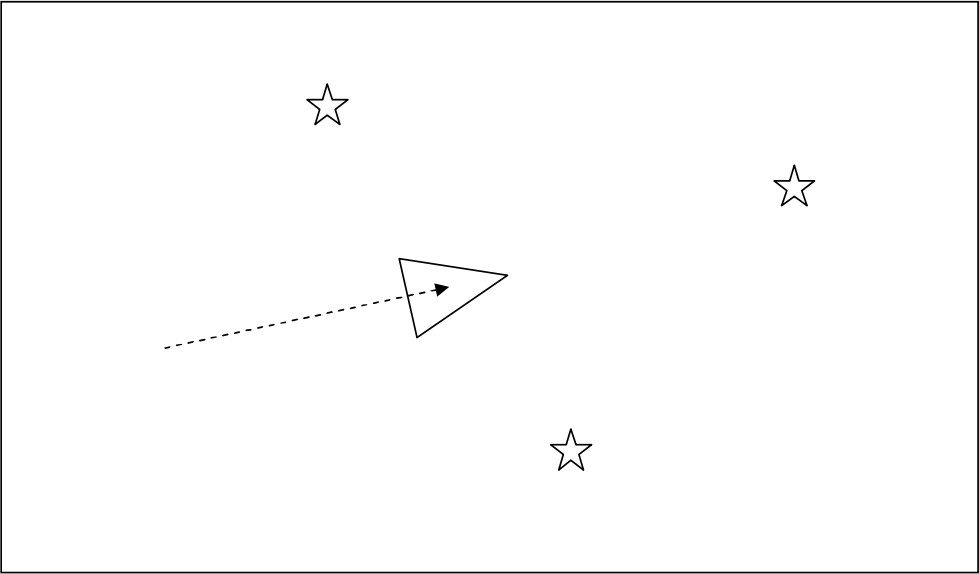
\includegraphics[height=\paperheight]{ekf0.png}}
    \begin{frame}{}
    \end{frame}
  }
  
  {
    \usebackgroundtemplate{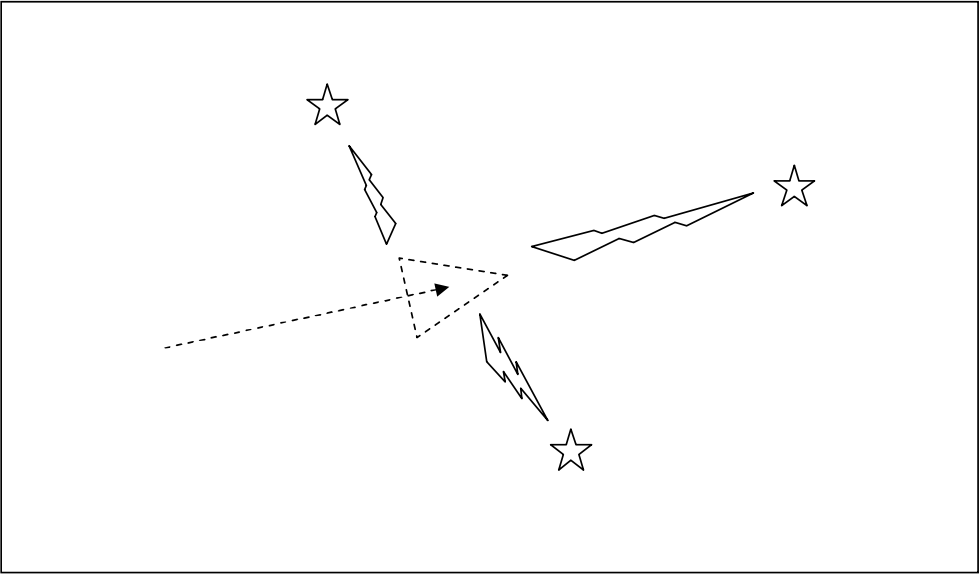
\includegraphics[height=\paperheight]{ekf1.png}}
    \begin{frame}{}
    \end{frame}
  }
  
  {
    \usebackgroundtemplate{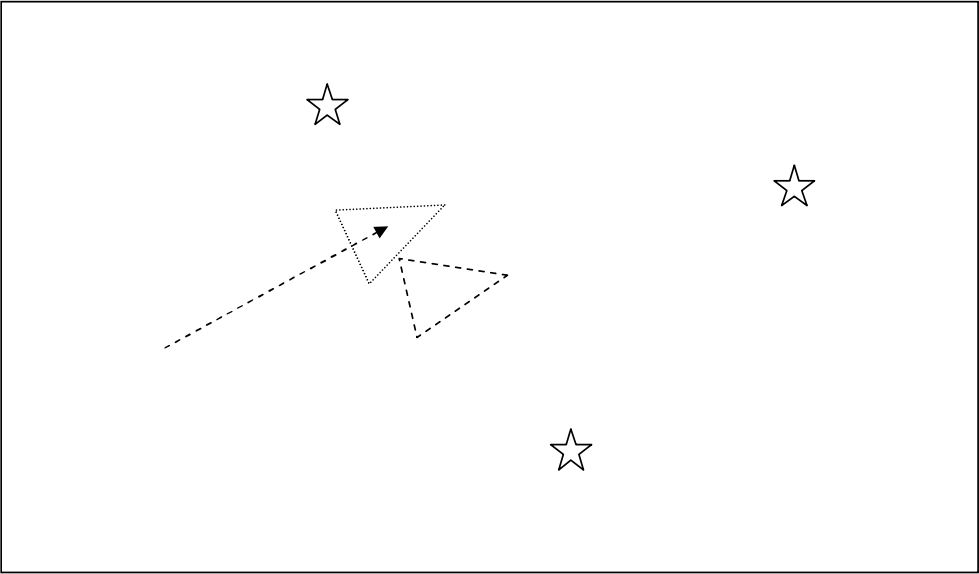
\includegraphics[height=\paperheight]{ekf2.png}}
    \begin{frame}{}
    \end{frame}
  }

  {
    \usebackgroundtemplate{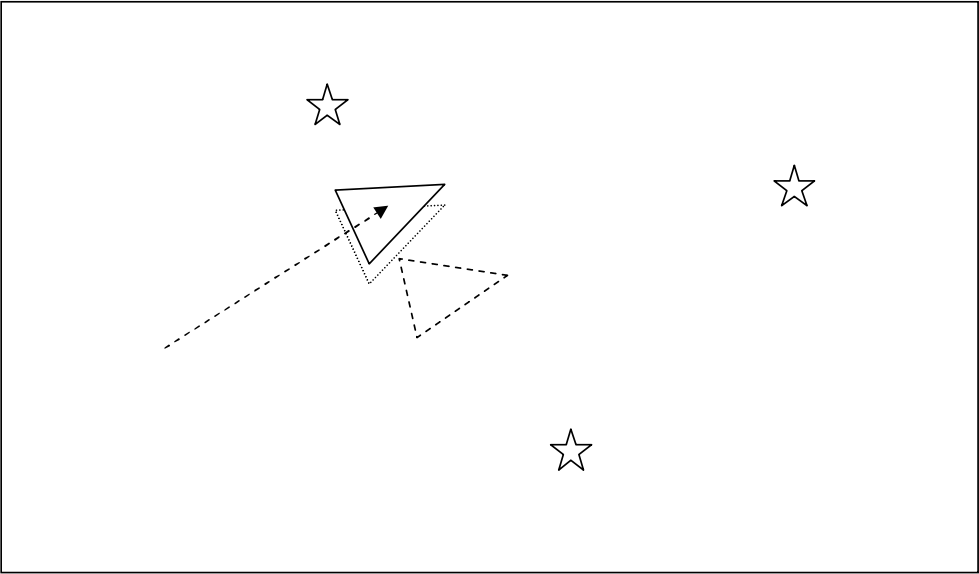
\includegraphics[height=\paperheight]{ekf3.png}}
    \begin{frame}{}
    \end{frame}
  }
  
  \section{Mapping}
  %----Mapping - Who?--------------------------------------------------%
  \begin{frame}{\bf Mapping}

    Idea: occupancy grid
    \vspace{1cm}

    \begin{itemize}
    \item The world is represented as a grid of cells, each cell holding a
          probability that it is occupied
    \item On every laser scan, the cells where the laser beams end get their
          values increased
    \end{itemize}
    \vspace{1cm}

    This relies on having accurate robot pose at all times.
  \end{frame}
  
  \section{Demo}
  %----Demo - Both--------------------------------------------------%
  \begin{frame}{\bf Demo}
    
  \end{frame}
  
  \section{Bibliography}
  %----Demo - Both--------------------------------------------------%
  \begin{frame}{\bf Bibliography}
    \begin{thebibliography}{3}

    \bibitem{SlamForDummies} Riisgaard \& Blas. MIT OpenCourseWare.
      \newblock \emph{``SLAM For Dummies''}.
      \newblock
      ``\url{http://ocw.mit.edu/courses/aeronautics-and-astronautics/
        16-412j-cognitive-robotics-spring-2005/projects/}''. 2004.
      
    \end{thebibliography}
  \end{frame}
  

\end{document}
